\chapter{单变量函数}
前面中我们已经说明了如何由量的度量而产生实数
系。在这一章中我们要进一步说明如何用变数符号去表达变
量,用变数之间的函数关系去表达变量之间的关联。变数是
变量的抽象,函数是变量相互关系的抽象。在这一章里我们
还要运用极限来分析和确立连续函数的概念。

\section{函数的概念}
\subsection{变数和变域}
在研究自然现象时,人们会遇到许多不同的物理量,如
时间、长度、体积、速度、质量、力等等。按照给定条件,
能取许多不同数值的量叫做\textbf{变量};而只取一个数值的量叫做
\textbf{常量},用来表达变量的符号叫做\textbf{变数}。习惯上常用$x,y,
z$等字母表示变数,从纯数学的观点来说,一个变数就是一
个“能取许多不同数值”的符号,它所能取的所有数值构成
一个集合,叫做它的\textbf{变域}。如果变数$x$的变域已经给出,我
们就认为变数$x$是已知的。一般说来,任何数集可以当作变
数的变域。常会遇到取所有自然数的变数$n$, 譬如数列中的
项数。可是在现实生活中,我们通常研究的是连续变化的变
数,如动点所经过的路程及所花的时间等物理量,就是这种
变数的原形,数的区间就是这一类变数的变域,最常用的区
间是以两个实数$a$与$b$ $(a<b)$——它的两个端点——为界
限的有限区间,两个端点本身可以包含在区间内,也可以不
包含在内。因此我们可以把区间分为:
\begin{itemize}
    \item 开区间$(a,b)$就是$\{x|a<x<b\}$;
    \item  闭区间$[a,b]$就是$\{x|a\le x\le b\}$;
    \item  半开区间$(a,b]$就是$\{x|a<x\le b\}$;
    $[a,b)$就是$\{x|a\le x<b\}$。
\end{itemize}
在上述各种情形,数$b-a$为区间的长度。

常量可以看作变量的特殊情形,它的变域是由一个数组
成的集合$\{x|x=a\}$。

数轴上的线段是数的区间的几何表示,图示开区间如图
8.1或8.2。

在点$a,b$处的圆圈或圆括号表示从区间去掉这两个
数。在两个圆圈之间的粗线段表示在$a,b$之间的一切数$x$。
图示闭区间如图8.3。
图示半开区间如图8.4、8.5,每一种情形都只包含出现
有方括号的数,以及在$a,b$之间的一切实数。
\begin{figure}[htp]\centering
    \begin{minipage}[t]{0.48\textwidth}
    \centering
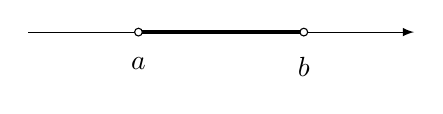
\begin{tikzpicture}[>=latex, scale=.7]
       \draw[->] (0.5,0)--(7.5,0);
       \draw[ultra thick] (2.5,0)node[below=5pt]{$a$}--(5.5,0)node[below=5pt]{$b$};
       \draw (2.5,0)[fill=white] circle (2pt);
        \draw (5.5,0)[fill=white] circle (2pt);
    \end{tikzpicture}
    \caption{}
    \end{minipage}
    \begin{minipage}[t]{0.48\textwidth}
    \centering
    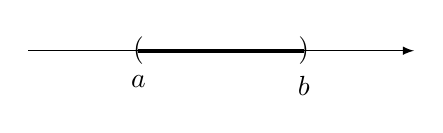
\begin{tikzpicture}[>=latex, scale=.7]
        \draw[->] (0.5,0)--(7.5,0);
        \draw[ultra thick] (2.5,0)node[below=5pt]{$a$}--(5.5,0)node[below=5pt]{$b$};
        \node at (2.5,0){$($}; \node at (5.5,0){$)$};
    \end{tikzpicture}
    \caption{}
    \end{minipage}
    \end{figure}

\begin{figure}[htp]\centering
    \begin{minipage}[t]{0.48\textwidth}
    \centering
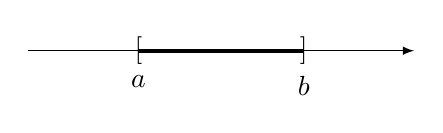
\begin{tikzpicture}[>=latex, scale=.7]
    \draw[->] (0.5,0)--(7.5,0);
    \draw[ultra thick] (2.5,0)node[below=5pt]{$a$}--(5.5,0)node[below=5pt]{$b$};
    \node at (2.5,0){$[$}; \node at (5.5,0){$]$};
    \end{tikzpicture}
    \caption{}
    \end{minipage}
    \begin{minipage}[t]{0.48\textwidth}
    \centering
    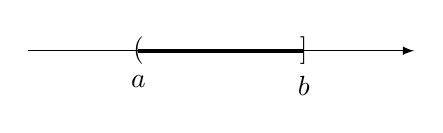
\begin{tikzpicture}[>=latex, scale=.7]
        \draw[->] (0.5,0)--(7.5,0);
        \draw[ultra thick] (2.5,0)node[below=5pt]{$a$}--(5.5,0)node[below=5pt]{$b$};
        \node at (2.5,0){$($}; \node at (5.5,0){$]$};
    \end{tikzpicture}
    \caption{}
    \end{minipage}
    \end{figure}

\begin{figure}[htp]\centering
    \begin{minipage}[t]{0.48\textwidth}
    \centering
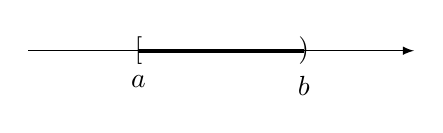
\begin{tikzpicture}[>=latex, scale=.7]
    \draw[->] (0.5,0)--(7.5,0);
    \draw[ultra thick] (2.5,0)node[below=5pt]{$a$}--(5.5,0)node[below=5pt]{$b$};
    \node at (2.5,0){$[$}; \node at (5.5,0){$)$};
    \end{tikzpicture}
    \caption{}
    \end{minipage}
    \begin{minipage}[t]{0.48\textwidth}
    \centering
    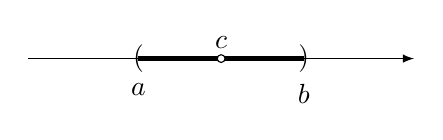
\begin{tikzpicture}[>=latex, scale=.7]
        \draw[->] (0.5,0)--(7.5,0);
        \draw[ultra thick] (2.5,0)node[below=5pt]{$a$}--(5.5,0)node[below=5pt]{$b$};
        \node at (2.5,0){$($}; \node at (5.5,0){$)$};
        \draw (4,0)[fill=white] circle (2pt)node[above]{$c$};
    \end{tikzpicture}
    \caption{}
    \end{minipage}
    \end{figure}

有时也要考虑无穷区间,用符号$-\infty,+\infty$作为一端或
两端,它们的记号和上面所引进的相类似,例如$(-\infty,+\infty)$
是全体实数集合$\{x|x\in\mathbb{R}\}$, 区间$(a,+\infty)$表示集
合$\{x|x>a\}$, 区间$(-\infty,b]$表示集合$\{x|x\le b\}$. 无穷区间
在几何上可用两端无限伸延的直线或一端无限伸延的射线来
表示。

以后我们要常用到一点的邻域的概念。\textbf{$c$点的邻域}是包
含$c$点的任何开区间$(a,b)$, 而$c$点的去心邻域指去掉$c$
点的任何$c$点的邻域。它的图象如图8.6。

$c$点的去心邻域可写成$(a,c)\cup (c,b)$. 我们常把
$c$点的邻域写成对称的形式:$(c-r,c+r)$, 对任何
$r>0$, 并且称它为\textbf{$c$点的对称邻域}。

\begin{example}
    试写出含于区间$(1,5)$中$\pi$的对称邻域。
$\left(\pi-\frac{1}{2},\pi+\frac{1}{2}\right)$是含于$(1,5)$的$\pi$对称邻域。此外
$(\pi-1,\pi+1)$, $\left(\pi-\frac{3}{2},\pi+\frac{3}{2}\right)$, $(\pi-0.01,\pi+0.01)$
等都是含于$(1,5)$中的对称邻域。
\end{example}

\subsection{函数的定义}
我们已经在第三册研究过许多函数,例如多项式函数、
三角函数,由于函数这个概念的重要性,并且它将是我们
的主要研究对象,因此需要回忆一般的函数的定义,下面我
们从数集之间的多对一(包括一对一)的关系重新给出函数
定义。

\begin{blk}{定义}
     设有数集$A,B$, 如果有一对应关系或法则$f$存
在,对于$A$的任何一个数$x$, 有数集$B$中唯一的一个数$y$与之
对应,我们就称给出了一个从数集$A$到数集$B$内的函数$f$, 用
\[f:A\mapsto B\]
表示,并写成$y=f(x),\; (x\in A)$, 此时称$f(x)$为函数$f$在$x$的
函数值,并称$A$为函数$f$的\textbf{定义域}。又当$x$取遍$A$中的数时,
函数值$f(x)$全体也构成一个数集,称为函数$f$的\textbf{值域},记作
\[f(A)=\{f(x)|x\in A\}\]
要注意的是在构造一个函数$f:A\mapsto B$的时候,$f(A)$不一定等
于$B$, 而是$B$的一个真子集,即$f(A)\subset B$。
\end{blk}



\begin{example}
设$\mathbb{R}$是实数集,函数$f:\mathbb{R}\mapsto\mathbb{R}$定义为
\[f(x)=\frac{2x}{x^2+1},\quad x\in(-\infty,+\infty)\]
求它的值域。
\end{example}

\begin{solution}
    方程$f(x)=\frac{2x}{x^2+1}$等价于
    \begin{equation}
        yx^2-2x+y=0
    \end{equation}
根据函数的值域定义,任给$y\in f(\mathbb{R})$, 方程(8.1)必有实数
解,而方程(8.1)有实数解的充要条件是
\[\Delta=1-y^2\ge 0\]
即:$-1\le y\le 1$,所以
\[f(\mathbb{R})=\{f(x)|-1\le f(x)\le 1\}\subset \mathbb{R}\]
\end{solution}

在函数的定义中包含三个要素,即\textbf{定义域},\textbf{多对一的对
应法则}和\textbf{函数值所在的数集}。应养成一个习惯,当给定一个
函数时,必须指明它的定义域。在实际问题中,函数的定义
域是根据实际意义来确定的,例如温度计刻有华氏温标度数
$F$和摄氏温标度数$c$,因为不存在低于绝对零度的温度,因
此,这两个度数之间的函数$\varphi$是
\[F=\varphi(c)=\frac{9}{5}c+32,\quad c\in (-273,+\infty)\]

以后,当我们只在数学上,一般地研究一个具体解析式
子规定的函数关系时,如果定义域$A$没有被指明,那么函数
的定义域是使解析式子具有数值意义的所有$x$的数值组成的
自然定义域,函数$y$的值域通常是不指出的,因为由对应的
规律本身就可以确定函数的值域。










\begin{example}
    
\end{example}

\begin{solution}
    
\end{solution}



\begin{solution}
    
\end{solution}







\begin{example}
    
\end{example}
\begin{solution}
    
\end{solution}

\begin{example}
    
\end{example}


\begin{solution}
    
\end{solution}

\begin{example}
    
\end{example}


\begin{solution}
    
\end{solution}


\begin{example}
    
\end{example}



\begin{solution}
    
\end{solution}


































